% !TEX TS-program = pdflatex
% !TEX encoding = UTF-8 Unicode

% This is a simple template for a LaTeX document using the "article" class.
% See "book", "report", "letter" for other types of document.

\documentclass[11pt]{article} % use larger type; default would be 10pt

\usepackage[utf8]{inputenc} % set input encoding (not needed with XeLaTeX)

%%% Examples of Article customizations
% These packages are optional, depending whether you want the features they provide.
% See the LaTeX Companion or other references for full information.

%%% PAGE DIMENSIONS
\usepackage{geometry} % to change the page dimensions
\geometry{a4paper} % or letterpaper (US) or a5paper or....
% \geometry{margin=2in} % for example, change the margins to 2 inches all round
% \geometry{landscape} % set up the page for landscape
%   read geometry.pdf for detailed page layout information

\usepackage{graphicx} % support the \includegraphics command and options
\usepackage{amsmath}
\usepackage{amsfonts}

% \usepackage[parfill]{parskip} % Activate to begin paragraphs with an empty line rather than an indent

%%% PACKAGES
\usepackage{booktabs} % for much better looking tables
\usepackage{array} % for better arrays (eg matrices) in maths
\usepackage{paralist} % very flexible & customisable lists (eg. enumerate/itemize, etc.)
\usepackage{verbatim} % adds environment for commenting out blocks of text & for better verbatim
\usepackage{subfig} % make it possible to include more than one captioned figure/table in a single float
% These packages are all incorporated in the memoir class to one degree or another...

%%% HEADERS & FOOTERS
\usepackage{fancyhdr} % This should be set AFTER setting up the page geometry
\pagestyle{fancy} % options: empty , plain , fancy
\renewcommand{\headrulewidth}{0pt} % customise the layout...
\lhead{}\chead{}\rhead{}
\lfoot{}\cfoot{\thepage}\rfoot{}

%%% SECTION TITLE APPEARANCE
\usepackage{sectsty}
\allsectionsfont{\sffamily\mdseries\upshape} % (See the fntguide.pdf for font help)
% (This matches ConTeXt defaults)

%%% ToC (table of contents) APPEARANCE
\usepackage[nottoc,notlof,notlot]{tocbibind} % Put the bibliography in the ToC
\usepackage[titles,subfigure]{tocloft} % Alter the style of the Table of Contents
\renewcommand{\cftsecfont}{\rmfamily\mdseries\upshape}
\renewcommand{\cftsecpagefont}{\rmfamily\mdseries\upshape} % No bold!

%%% END Article customizations

%%% The "real" document content comes below...

\title{Computational Stochastic Processes - Project 3}
\author{Tom McGrath}
%\date{} % Activate to display a given date or no date (if empty),
         % otherwise the current date is printed 

\begin{document}
\maketitle

\section{Q1}

\subsection{Q1.i.}

We wish to calculate the expectation of a function with respect to a probability distribution $\pi(x)$, $x \in \mathbb{R}^{d}$ using a diffusion process of form:

\begin{equation}
	dX_{t} = -\nabla V(X_{t})dt + \sqrt{2}dW_{t}
\end{equation}

The aim is to set the diffusion process up so that the invariant distribution of $X_{t}$ is $\pi(x)$. For this to be the case, we need the probability measure to be invariant under the dynamics of the diffusion process, which is the case is the following equation is satisfied:

\begin{equation}
	P^{*}_{t} \pi = \pi
\end{equation}

where the semigroup $P^{*}_{t}$ generated by the adjoint of the generator $\mathcal{L}^{*}$ is:

\begin{equation}
	P^{*}_{t} = \exp(\mathcal{L}^{*}t)
\end{equation}

if there is a unique invariant measure then the dynamics from the diffusion process are ergodic and we can take the long-time limit to find our expectation:

\begin{equation}
	\lim_{T\to\infty}\frac{1}{T}\int^{T}_{0}f(X_{s})ds = \int_{\mathbb{R}^{d}}f(x)\pi(x)dx
\end{equation}

as we wanted.

\subsection{Q1.ii.}
Initially I was unsure how to do this, so searched the literature and discovered a similar approach using what is essentially a diffusion process by Garcia-Cortes and Cabrillo (A Monte Carlo algorithm for efficient large matrix inversion, 2008 on arXiV). By considering the matrix $C$ that we wish to invert as the covariance matrix of a multivariate normal distribution

\begin{equation}
	z \sim \mathcal{N}(0,C^{-1})
\end{equation}

we can draw using a stochastic process for $z$. At step $k$:

\begin{equation}
	z_{i}^{k} = \phi^{k}\frac{1}{\sqrt{c_{ii}}} - \frac{1}{c_{ii}}\sum^{i-1}_{j=1}z^{k}_{i-1}c_{ij} - \frac{1}{c_{ii}}\sum^{n}_{j=i1}z^{k-1}_{i-1}c_{ij}
\end{equation}

Now we can estimate the inverse matrix:

\begin{equation}
	\mathbb{E}(z z^{T}) = C^{-1}
\end{equation}

Alternatively, we could use a stationary OU process:

\begin{equation}
	d\mathbf{X}_{t} = -\mathbf{C}\mathbf{X}_{t}dt + d\mathbf{W}_{t}
\end{equation}

where $\mathbf{C}$ is the matrix we wish to invert. We can then use a maximum likelihood estimator approach as in slide 198 of the lecture notes to estimate the inverse matrix.

\subsection{Q1.iii}
Code is attached at the end of the file. Z is the estimated inverse of C. The exact inverse is printed last.
\footnotesize
\begin{verbatim}
C =

    0.4950    0.3032    0.3583    0.4604    0.2044    0.4621    0.6109    0.5435    0.3352    0.4904
    0.3032    0.4582    0.3662    0.4022    0.1711    0.5557    0.5101    0.4424    0.3885    0.4152
    0.3583    0.3662    0.5646    0.4878    0.2897    0.5080    0.5899    0.6184    0.3896    0.5316
    0.4604    0.4022    0.4878    0.5590    0.2863    0.5237    0.6722    0.6152    0.4284    0.5620
    0.2044    0.1711    0.2897    0.2863    0.3749    0.3298    0.4542    0.4692    0.2559    0.4408
    0.4621    0.5557    0.5080    0.5237    0.3298    0.8939    0.7601    0.7357    0.4579    0.6283
    0.6109    0.5101    0.5899    0.6722    0.4542    0.7601    1.0000    0.8756    0.5975    0.7677
    0.5435    0.4424    0.6184    0.6152    0.4692    0.7357    0.8756    0.8867    0.5221    0.8125
    0.3352    0.3885    0.3896    0.4284    0.2559    0.4579    0.5975    0.5221    0.5922    0.5513
    0.4904    0.4152    0.5316    0.5620    0.4408    0.6283    0.7677    0.8125    0.5513    0.8717


Z =

   1.0e+04 *

    0.0052    0.0002    0.0039   -0.0041    0.0038    0.0009   -0.0003   -0.0069    0.0002    0.0011
    0.0002    0.2956   -0.2764    0.0257   -0.0198   -0.2251   -0.2615    0.7076    0.0502   -0.2776
    0.0039   -0.2764    0.2643   -0.0290    0.0217    0.2116    0.2469   -0.6720   -0.0478    0.2626
   -0.0041    0.0257   -0.0290    0.0078   -0.0045   -0.0206   -0.0248    0.0700    0.0048   -0.0266
    0.0038   -0.0198    0.0217   -0.0045    0.0051    0.0161    0.0174   -0.0538   -0.0033    0.0196
    0.0009   -0.2251    0.2116   -0.0206    0.0161    0.1721    0.1994   -0.5415   -0.0384    0.2121
   -0.0003   -0.2615    0.2469   -0.0248    0.0174    0.1994    0.2349   -0.6313   -0.0458    0.2480
   -0.0069    0.7076   -0.6720    0.0700   -0.0538   -0.5415   -0.6313    1.7158    0.1223   -0.6715
    0.0002    0.0502   -0.0478    0.0048   -0.0033   -0.0384   -0.0458    0.1223    0.0096   -0.0484
    0.0011   -0.2776    0.2626   -0.0266    0.0196    0.2121    0.2480   -0.6715   -0.0484    0.2639


ans =

   1.0e+04 *

    0.0050    0.0011    0.0027   -0.0038    0.0035    0.0001   -0.0011   -0.0041    0.0004    0.0001
    0.0011    0.2473   -0.2300    0.0205   -0.0156   -0.1880   -0.2184    0.5896    0.0418   -0.2316
    0.0027   -0.2300    0.2195   -0.0238    0.0175    0.1759    0.2054   -0.5582   -0.0398    0.2184
   -0.0038    0.0205   -0.0238    0.0071   -0.0039   -0.0165   -0.0201    0.0569    0.0039   -0.0216
    0.0035   -0.0156    0.0175   -0.0039    0.0046    0.0128    0.0138   -0.0433   -0.0025    0.0156
    0.0001   -0.1880    0.1759   -0.0165    0.0128    0.1435    0.1662   -0.4506   -0.0320    0.1767
   -0.0011   -0.2184    0.2054   -0.0201    0.0138    0.1662    0.1964   -0.5258   -0.0383    0.2069
   -0.0041    0.5896   -0.5582    0.0569   -0.0433   -0.4506   -0.5258    1.4264    0.1019   -0.5589
    0.0004    0.0418   -0.0398    0.0039   -0.0025   -0.0320   -0.0383    0.1019    0.0081   -0.0405
    0.0001   -0.2316    0.2184   -0.0216    0.0156    0.1767    0.2069   -0.5589   -0.0405    0.2200
\end{verbatim}
\normalsize
For Gauss-Jordan elimination, the computational cost for matrix inversion is $\mathcal{O}(n^{3})$. This algorithm is (according to the authors) linear in the number of nonzero elements to invert - however this only counts running the algorithm for one step. To obtain accuracy, many steps are needed, although this is a function of the desired accuracy rather than the matrix size, so presents an advantage when exact precision is not necessary but the matrix under consideration is very large. The algorithm is also highly parallelisable, which is another computational advantage (although exact matrix inversion is also parallelisable).

\subsection{Q1.iv}
We require the SDE to be ergodic, so Hasminski's criterion must be satisfied, i.e. $-\nabla V(X^{b}_{t}) + b(X^{b}_{t})$ must be smooth (we know the $-\nabla V(X^{b}_{t})$ term is smooth, so simply require that $b(X^{b}_{t})$ is also smooth). We then require that:

\begin{equation}
\langle -\nabla V(X^{b}_{t}) + b(X^{b}_{t}), x \rangle \leq -\beta|x|^{2}
\end{equation}

We also require the same condition with the forward Kolmogorov equation as before.

\section{Q2}
\subsection{Q2.i.}
In general the likelihood is given by:

\begin{equation}
L(X_{t};\theta, T) = \exp\left(\int^{T}_{0}b(X_{s};\theta)dX_{s} - \frac{1}{2}\int^{T}_{0}(b(X_{s};\theta))^{2}dx\right)
\end{equation}

and the log-likelihood is given by:

\begin{equation}
l = \int^{T}_{0}b(X_{s};\theta)dX_{s} - \frac{1}{2}\int^{T}_{0}(b(X_{s};\theta))^{2}dx
\end{equation}

so in this case the log-likelihood is given by:

\begin{equation}
	l = \int^{T}_{0}\sum^{N}_{j=1}\theta_{j}f'_{j}(X_{s})dX_{s} - \frac{1}{2}\int^{T}_{0}(\sum^{N}_{j=1}\theta_{j}f'_{j}(X_{s}))^{2}ds
\end{equation}

To obtain maximum likelihood estimators we need to differentiate with respect to each $\theta$, obtain a linear system of equation and solve for the MLE. Expanding the squared sum we obtain:

\begin{equation}
	l = \int^{T}_{0}\sum^{N}_{j=1}\theta_{j}f'_{j}(X_{s})dX_{s} -\frac{1}{2}\int^{T}_{0}\sum^{N}_{i=1}\sum^{N}_{j=1}\theta_{i}\theta_{j}f'_{i}(X_{s})f'_{j}(X_{s})ds
\end{equation}

Differentiating with respect to $\theta_{k}$:

\begin{equation}
 \frac{\partial l}{\partial \theta_{k}} = \int^{T}_{0}f'_{k}(X_{s})dX_{s} - \frac{1}{2}\int^{T}_{0}\sum^{N}_{i\neq k}\theta_{i}f'_{i}(X_{s})f'_{k}(X_{s})ds - \int^{T}_{0}\theta_{k}(f'_{k}(X_{s}))^{2}ds = 0
\end{equation}

When $N$ and $f_{i}$ are known, we can rearrange these into a system of equations similar to those on slide 184 of the lecture notes.

\subsection{Q2.ii.}
I generated a path according to the SDE via the Euler-Marayama scheme with a time step of $\delta t = 0.01$ and $\theta$ as provided in the question. Inserting the quartic potential functions into the expression for the log-likelihood I obtained:

\begin{align}
	l &= \int^{T}_{0}4\theta_{4}X_{s}^{3}+3\theta_{3}X_{s}^{2}+2\theta_{2}X_{s}+\theta_{1}\\
	&-\frac{1}{2}\int^{T}_{0}16\theta_{4}^{2}X_{s}^{6}+24\theta_{4}\theta_{3}X_{s}^{5}+16\theta_{4}\theta_{2}X_{s}^{4}
+8\theta_{4}\theta_{1}X_{s}^{3}ds\\
&-\frac{1}{2}\int^{T}_{0}9\theta_{3}^{2}X_{s}^{4}+12\theta_{3}\theta_{2}X_{s}^{3}+6\theta_{3}\theta_{1}X_{s}^{2}\\
&-\frac{1}{2}\int^{T}_{0}4\theta_{2}^{2}X_{s}^{2}+4\theta_{2}\theta_{1}X_{s}+\theta_{1}^{2}ds
\end{align}

Minimising these with respect to each $\theta_{i}$ gives the following system of equations (following the conventions set out on slide 178 of the lecture notes):

\begin{equation}
\begin{bmatrix} M_{0} & 2M_{1} & 3M_{2} & 4M_{3}\\M_{1} & 2M_{2} & 3M_{3} & 4M_{4}\\M_{2} & 2M_{3} & 3M_{4} & 4M_{5}\\M_{3} & 2M_{4} & 3M_{5} & 4M_{6}\end{bmatrix}\begin{bmatrix}\theta_{1} \\ \theta_{2}\\ \theta_{3} \\ \theta{4}\end{bmatrix} = \begin{bmatrix}B_{0}\\B_{1}\\B_{2}\\B_{3}\end{bmatrix}
\end{equation}

Inverting this using MATLAB's symbolic toolbox creates enormous expressions for each estimator for $\theta$ which, unsurprisingly, give the wrong answer! Therefore I must have made a mistake somewhere in the derivation. I also coded the quadratic variation estimator of the diffusion coefficient given on slide 168, but only recovered $\sigma = 0.25$ rather than $0.5$ as expected.

\subsection{Q2.iii}
This is a 1D process, so as long as the conditions set out in Ait-Sahalia's paper are satisfied, we can use the Lamperti transform to convert the process with multiplicative noise into one with additive noise. The transformation factor will be $h(x) = log(X_{s}$. We should now be able to calculate the coefficients using the same approach as above, obtaining new expressions for $\theta$.

\section{Q3}
\subsection{Q3.i. and ii.}
I used the long-time average and Euler discretisation to compute the mean, 2nd and 4th stationary moments of the distribution

\begin{equation}
	dX_{t} = -X_{t}dt+dW_{t},\quad X_{0} = 0
\end{equation}

This gives the results:
\begin{figure}[h!]
\centering
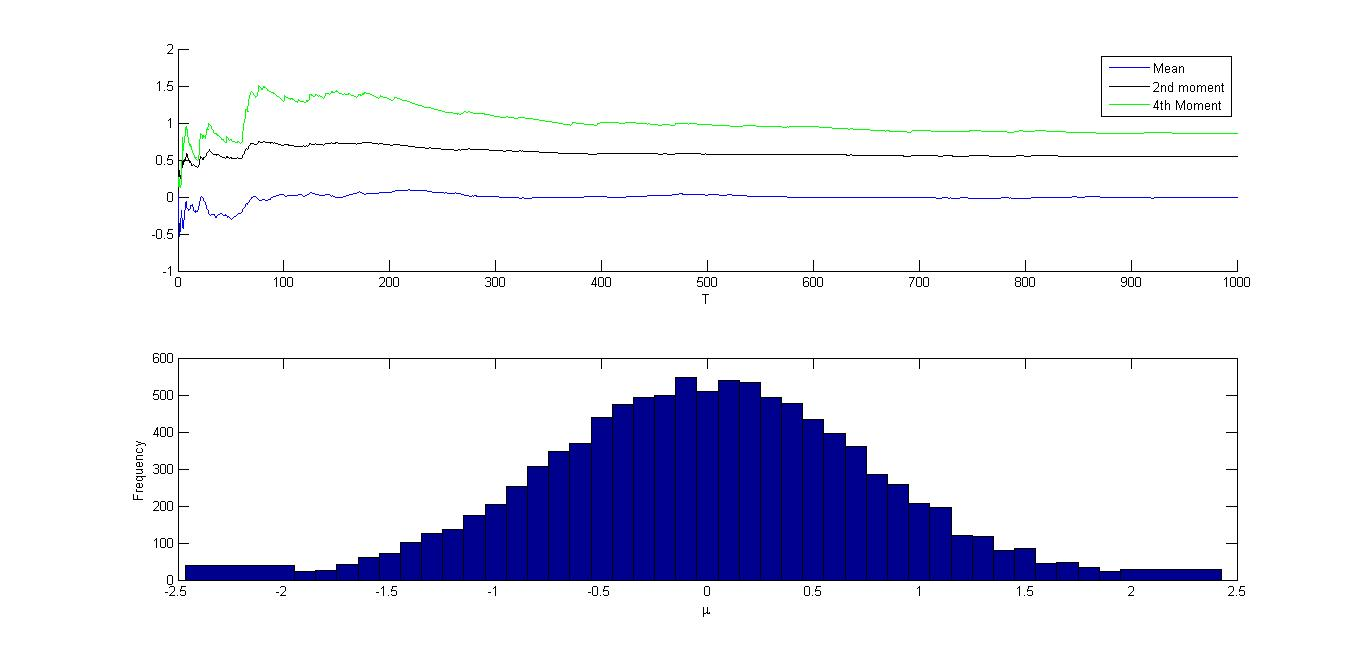
\includegraphics[width=0.9\textwidth]{q3i.jpg}
\caption{Probability density and moments for distribution 1}
\end{figure}

\subsection{Q3.iii}
For the distribution:

\begin{equation}
	dX_{t} = (X_{t} - X_{t}^{3})dx + dW_{t}
\end{equation}
we obtain the results:
\begin{figure}[h!]
\centering
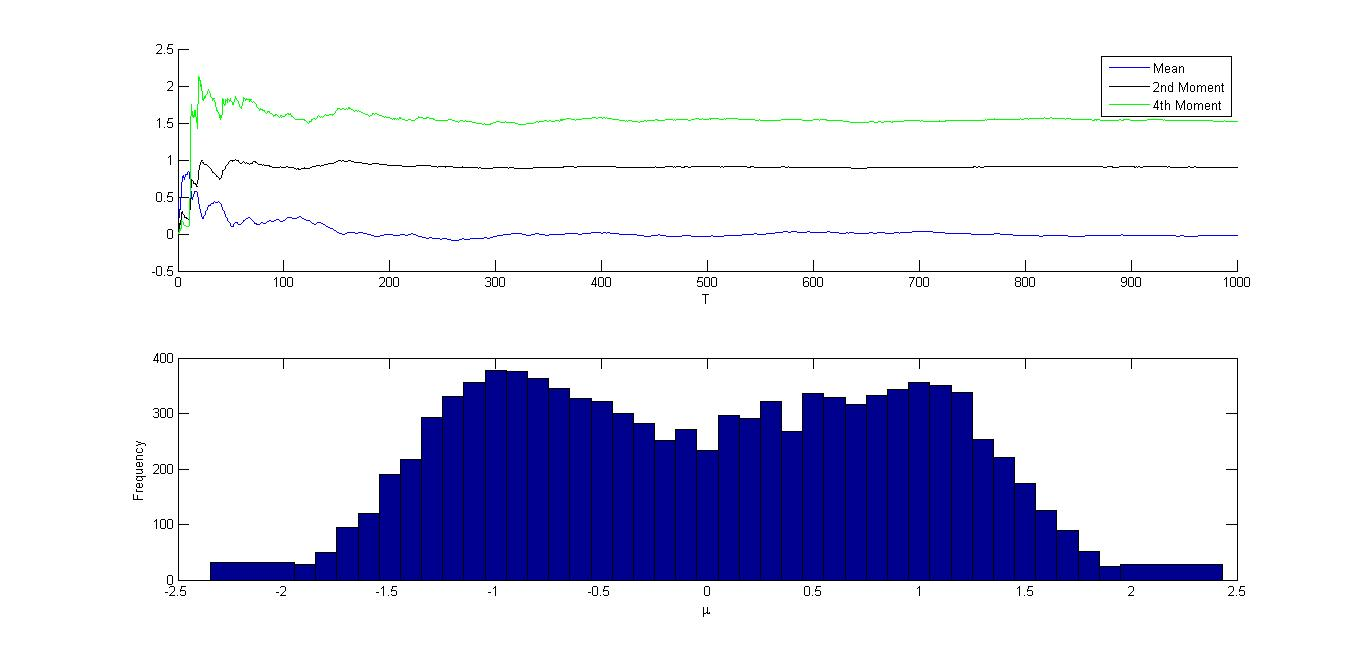
\includegraphics[width=0.9\textwidth]{q3iii.jpg}
\caption{Probability density and moments for distribution 2}
\end{figure}

\section{Code}
\subsection{Q1}
\begin{verbatim}clear all
clc

Tmax = 10000;
dt = 0.1;
dim = 10;
T = linspace(0,Tmax,Tmax/dt);

dW = randn(dim,length(T));
C = unifrnd(0,1,dim,dim);
C = C*C';
C = C./(max(max(C))+0.00000001);
X = zeros(dim, length(T));
Z = zeros(dim,dim);

%for i = 1:length(T)
%X(:,i) = mvnrnd(zeros(dim,1),C);
%end
Y = inv(C);

for k = 2:length(T)
    for i = 1:dim
        X(i,k) = dW(i,k)/sqrt(C(i,i));
        for j = 1:i-1
            X(i,k) = X(i,k) - (1/C(i,i))*X(j,k)*C(i,j);
        end
        
        for j = i+1:dim
            X(i,k) = X(i,k) - (1/C(i,i))*X(j,k-1)*C(i,j);
        end
    end
    k
end

for i = 1:length(T)
    Z = Z + (X(:,i)*transpose(X(:,i)));
end

Z = Z./length(T);
Z
inv(C)
\end{verbatim}

\subsection{Q2}
\begin{verbatim}
clear all
clc

Tmax = 10000;
dt = 0.01;
T = linspace(0, Tmax, Tmax/dt);

dW = dt*randn(1, length(T));
X = zeros(1,length(T));

X(1) = 0.0;

for i = 2:length(T)
    X(i) = X(i-1) - (8*X(i-1)^3 - 3*X(i-1)^2 - X(i-1) + 0.5)*dt + 0.5*dW(i);
end

M0 = dt;
M1 = sum(X)*dt;
M2 = sum(X.^2)*dt;
M3 = sum(X.^3)*dt;
M4 = sum(X.^4)*dt;
M5 = sum(X.^5)*dt;
M6 = sum(X.^6)*dt;
B0 = sum(diff(X));
B1 = sum(X(1:end-1).*diff(X));
B2 = sum((X(1:end-1).^2).*diff(X));
B3 = sum((X(1:end-1).^3).*diff(X));

S1 = (B0*(M6*M3^2 - 2*M3*M4*M5 + M4^3 - M2*M6*M4 + M2*M5^2))/(M6*M1^2*M4 - M1^2*M5^2 - 2*M6*M1*M2*M3 + 2*M1*M2*M4*M5 + 2*M1*M3^2*M5 - 2*M1*M3*M4^2 + M6*M2^3 - 2*M2^2*M3*M5 - M2^2*M4^2 + 3*M2*M3^2*M4 - M0*M6*M2*M4 + M0*M2*M5^2 - M3^4 + M0*M6*M3^2 - 2*M0*M3*M4*M5 + M0*M4^3) - (B1*(- M3^2*M5 + M3*M4^2 + M2*M6*M3 - M2*M4*M5 - M1*M6*M4 + M1*M5^2))/(M6*M1^2*M4 - M1^2*M5^2 - 2*M6*M1*M2*M3 + 2*M1*M2*M4*M5 + 2*M1*M3^2*M5 - 2*M1*M3*M4^2 + M6*M2^3 - 2*M2^2*M3*M5 - M2^2*M4^2 + 3*M2*M3^2*M4 - M0*M6*M2*M4 + M0*M2*M5^2 - M3^4 + M0*M6*M3^2 - 2*M0*M3*M4*M5 + M0*M4^3) - (B3*(M5*M2^2 - 2*M2*M3*M4 + M3^3 - M1*M5*M3 + M1*M4^2))/(M6*M1^2*M4 - M1^2*M5^2 - 2*M6*M1*M2*M3 + 2*M1*M2*M4*M5 + 2*M1*M3^2*M5 - 2*M1*M3*M4^2 + M6*M2^3 - 2*M2^2*M3*M5 - M2^2*M4^2 + 3*M2*M3^2*M4 - M0*M6*M2*M4 + M0*M2*M5^2 - M3^4 + M0*M6*M3^2 - 2*M0*M3*M4*M5 + M0*M4^3) - (B2*(- M6*M2^2 + M5*M2*M3 + M2*M4^2 - M3^2*M4 + M1*M6*M3 - M1*M5*M4))/(M6*M1^2*M4 - M1^2*M5^2 - 2*M6*M1*M2*M3 + 2*M1*M2*M4*M5 + 2*M1*M3^2*M5 - 2*M1*M3*M4^2 + M6*M2^3 - 2*M2^2*M3*M5 - M2^2*M4^2 + 3*M2*M3^2*M4 - M0*M6*M2*M4 + M0*M2*M5^2 - M3^4 + M0*M6*M3^2 - 2*M0*M3*M4*M5 + M0*M4^3)
S2 = (B1*(M6*M2^2 - 2*M2*M3*M5 + M4*M3^2 + M0*M5^2 - M0*M4*M6))/(2*M6*M1^2*M4 - 2*M1^2*M5^2 - 4*M6*M1*M2*M3 + 4*M1*M2*M4*M5 + 4*M1*M3^2*M5 - 4*M1*M3*M4^2 + 2*M6*M2^3 - 4*M2^2*M3*M5 - 2*M2^2*M4^2 + 6*M2*M3^2*M4 - 2*M0*M6*M2*M4 + 2*M0*M2*M5^2 - 2*M3^4 + 2*M0*M6*M3^2 - 4*M0*M3*M4*M5 + 2*M0*M4^3) + (B3*(- M2^2*M4 + M2*M3^2 + M1*M5*M2 - M1*M3*M4 - M0*M5*M3 + M0*M4^2))/(2*M6*M1^2*M4 - 2*M1^2*M5^2 - 4*M6*M1*M2*M3 + 4*M1*M2*M4*M5 + 4*M1*M3^2*M5 - 4*M1*M3*M4^2 + 2*M6*M2^3 - 4*M2^2*M3*M5 - 2*M2^2*M4^2 + 6*M2*M3^2*M4 - 2*M0*M6*M2*M4 + 2*M0*M2*M5^2 - 2*M3^4 + 2*M0*M6*M3^2 - 4*M0*M3*M4*M5 + 2*M0*M4^3) - (B0*(- M3^2*M5 + M3*M4^2 + M2*M6*M3 - M2*M4*M5 - M1*M6*M4 + M1*M5^2))/(2*M6*M1^2*M4 - 2*M1^2*M5^2 - 4*M6*M1*M2*M3 + 4*M1*M2*M4*M5 + 4*M1*M3^2*M5 - 4*M1*M3*M4^2 + 2*M6*M2^3 - 4*M2^2*M3*M5 - 2*M2^2*M4^2 + 6*M2*M3^2*M4 - 2*M0*M6*M2*M4 + 2*M0*M2*M5^2 - 2*M3^4 + 2*M0*M6*M3^2 - 4*M0*M3*M4*M5 + 2*M0*M4^3) - (B2*(M3^3 - M0*M3*M6 + M0*M4*M5 + M1*M2*M6 - M1*M3*M5 - M2*M3*M4))/(2*M6*M1^2*M4 - 2*M1^2*M5^2 - 4*M6*M1*M2*M3 + 4*M1*M2*M4*M5 + 4*M1*M3^2*M5 - 4*M1*M3*M4^2 + 2*M6*M2^3 - 4*M2^2*M3*M5 - 2*M2^2*M4^2 + 6*M2*M3^2*M4 - 2*M0*M6*M2*M4 + 2*M0*M2*M5^2 - 2*M3^4 + 2*M0*M6*M3^2 - 4*M0*M3*M4*M5 + 2*M0*M4^3)
S3 = (B2*(M6*M1^2 - 2*M1*M3*M4 + M2*M3^2 + M0*M4^2 - M0*M2*M6))/(3*M6*M1^2*M4 - 3*M1^2*M5^2 - 6*M6*M1*M2*M3 + 6*M1*M2*M4*M5 + 6*M1*M3^2*M5 - 6*M1*M3*M4^2 + 3*M6*M2^3 - 6*M2^2*M3*M5 - 3*M2^2*M4^2 + 9*M2*M3^2*M4 - 3*M0*M6*M2*M4 + 3*M0*M2*M5^2 - 3*M3^4 + 3*M0*M6*M3^2 - 6*M0*M3*M4*M5 + 3*M0*M4^3) + (B3*(- M5*M1^2 + M4*M1*M2 + M1*M3^2 - M2^2*M3 + M0*M5*M2 - M0*M4*M3))/(3*M6*M1^2*M4 - 3*M1^2*M5^2 - 6*M6*M1*M2*M3 + 6*M1*M2*M4*M5 + 6*M1*M3^2*M5 - 6*M1*M3*M4^2 + 3*M6*M2^3 - 6*M2^2*M3*M5 - 3*M2^2*M4^2 + 9*M2*M3^2*M4 - 3*M0*M6*M2*M4 + 3*M0*M2*M5^2 - 3*M3^4 + 3*M0*M6*M3^2 - 6*M0*M3*M4*M5 + 3*M0*M4^3) - (B0*(- M6*M2^2 + M5*M2*M3 + M2*M4^2 - M3^2*M4 + M1*M6*M3 - M1*M5*M4))/(3*M6*M1^2*M4 - 3*M1^2*M5^2 - 6*M6*M1*M2*M3 + 6*M1*M2*M4*M5 + 6*M1*M3^2*M5 - 6*M1*M3*M4^2 + 3*M6*M2^3 - 6*M2^2*M3*M5 - 3*M2^2*M4^2 + 9*M2*M3^2*M4 - 3*M0*M6*M2*M4 + 3*M0*M2*M5^2 - 3*M3^4 + 3*M0*M6*M3^2 - 6*M0*M3*M4*M5 + 3*M0*M4^3) - (B1*(M3^3 - M0*M3*M6 + M0*M4*M5 + M1*M2*M6 - M1*M3*M5 - M2*M3*M4))/(3*M6*M1^2*M4 - 3*M1^2*M5^2 - 6*M6*M1*M2*M3 + 6*M1*M2*M4*M5 + 6*M1*M3^2*M5 - 6*M1*M3*M4^2 + 3*M6*M2^3 - 6*M2^2*M3*M5 - 3*M2^2*M4^2 + 9*M2*M3^2*M4 - 3*M0*M6*M2*M4 + 3*M0*M2*M5^2 - 3*M3^4 + 3*M0*M6*M3^2 - 6*M0*M3*M4*M5 + 3*M0*M4^3)
S4 = (B2*(- M5*M1^2 + M4*M1*M2 + M1*M3^2 - M2^2*M3 + M0*M5*M2 - M0*M4*M3))/(4*M6*M1^2*M4 - 4*M1^2*M5^2 - 8*M6*M1*M2*M3 + 8*M1*M2*M4*M5 + 8*M1*M3^2*M5 - 8*M1*M3*M4^2 + 4*M6*M2^3 - 8*M2^2*M3*M5 - 4*M2^2*M4^2 + 12*M2*M3^2*M4 - 4*M0*M6*M2*M4 + 4*M0*M2*M5^2 - 4*M3^4 + 4*M0*M6*M3^2 - 8*M0*M3*M4*M5 + 4*M0*M4^3) + (B1*(- M2^2*M4 + M2*M3^2 + M1*M5*M2 - M1*M3*M4 - M0*M5*M3 + M0*M4^2))/(4*M6*M1^2*M4 - 4*M1^2*M5^2 - 8*M6*M1*M2*M3 + 8*M1*M2*M4*M5 + 8*M1*M3^2*M5 - 8*M1*M3*M4^2 + 4*M6*M2^3 - 8*M2^2*M3*M5 - 4*M2^2*M4^2 + 12*M2*M3^2*M4 - 4*M0*M6*M2*M4 + 4*M0*M2*M5^2 - 4*M3^4 + 4*M0*M6*M3^2 - 8*M0*M3*M4*M5 + 4*M0*M4^3) + (B3*(M4*M1^2 - 2*M1*M2*M3 + M2^3 - M0*M4*M2 + M0*M3^2))/(4*M6*M1^2*M4 - 4*M1^2*M5^2 - 8*M6*M1*M2*M3 + 8*M1*M2*M4*M5 + 8*M1*M3^2*M5 - 8*M1*M3*M4^2 + 4*M6*M2^3 - 8*M2^2*M3*M5 - 4*M2^2*M4^2 + 12*M2*M3^2*M4 - 4*M0*M6*M2*M4 + 4*M0*M2*M5^2 - 4*M3^4 + 4*M0*M6*M3^2 - 8*M0*M3*M4*M5 + 4*M0*M4^3) - (B0*(M5*M2^2 - 2*M2*M3*M4 + M3^3 - M1*M5*M3 + M1*M4^2))/(4*M6*M1^2*M4 - 4*M1^2*M5^2 - 8*M6*M1*M2*M3 + 8*M1*M2*M4*M5 + 8*M1*M3^2*M5 - 8*M1*M3*M4^2 + 4*M6*M2^3 - 8*M2^2*M3*M5 - 4*M2^2*M4^2 + 12*M2*M3^2*M4 - 4*M0*M6*M2*M4 + 4*M0*M2*M5^2 - 4*M3^4 + 4*M0*M6*M3^2 - 8*M0*M3*M4*M5 + 4*M0*M4^3)

sig = (1/(dt*Tmax))*sum(diff(X).^2)
\end{verbatim}

\subsection{Q3}
\begin{verbatim}
clear all
clc

Tmax = 1000;
dt = 0.1;
epsilon = 0.1;

T = linspace(0,Tmax,Tmax/dt);
X = zeros(1,length(T));
dW = randn(1,length(T));
m = zeros(1,length(T));
v = zeros(1,length(T));
k = zeros(1,length(T));
Y = linspace(-2,2,41);

X(1) = 0.0;
for i = 2:length(T)
    % part i
    %X(i) = X(i-1) - X(i-1)*dt + sqrt(dt)*dW(i);
    % part iii
    X(i) = X(i-1) + (X(i-1)-X(i-1)^3)*dt + sqrt(dt)*dW(i);
end

for j = 1:length(T)
    m(j) = mean(X(1:j));
    v(j) = moment(X(1:j),2);
    k(j) = moment(X(1:j),4);
    j
end

figure
subplot(2,1,1);
hold on
    plot(T,m)
    plot(T,v, 'Color', 'black')
    plot(T,k, 'Color', 'green')
hold off

subplot(2,1,2);
hist(X,Y)
\end{verbatim}



\end{document}
